%!TEX option = --shell-escape
\documentclass[parskip=half]{scrartcl}

\usepackage[utf8]{inputenc}
\usepackage[T1]{fontenc}
\usepackage{microtype}
\usepackage[sfdefault,scale=0.85]{FiraSans}
\usepackage[scale=0.85]{FiraMono}

\usepackage[ngerman]{babel}
\usepackage[babel,german=quotes]{csquotes}
\usepackage{tabularx}
\usepackage{xltabular}
\usepackage[table,xcdraw]{xcolor}
\usepackage{graphicx}
\usepackage{svg}
\usepackage{datetime}
\usepackage{multirow}
\usepackage[hidelinks]{hyperref}
\usepackage{tikz}
\usepackage{pgfplots}
\usepackage{wrapfig}
\usepackage{pgfplotstable}
\usetikzlibrary{positioning,matrix,calc,shapes.misc}
\usepackage{comment}
\usepackage[german]{varioref}
\usepackage[german]{cleveref}
\usepackage[shortlabels]{enumitem}
\usepackage{booktabs}
\usepackage{suffix}
\usepackage{multicol}
\usepackage{xparse}
\usepackage{pdflscape}
\usepackage[headsepline,footsepline]{scrlayer-scrpage}
\clearpairofpagestyles

\renewcommand\sectionlinesformat[4]{%
  \makebox[0pt][r]{#3}#4%
}

\newcolumntype{Y}{>{\raggedright\let\newline\\\arraybackslash\hspace{0pt}}X}

\definecolor{matrixgreen}{HTML}{008F11}
\let\originalhref\href
\renewcommand\href[2]{\originalhref{#1}{\color{matrixgreen}{#2}}}%

\usepackage{listings}
\lstset{ 
  basicstyle=\scriptsize\ttfamily,
  breakatwhitespace=false,
  breaklines=true,
  captionpos=b,
  commentstyle=\color{green!50!black},
  keepspaces=true,
  keywordstyle=\color{blue},
  numbers=left,
  numbersep=5pt,
  numberstyle=\scriptsize\ttfamily,
  showspaces=false,
  showstringspaces=false,
  showtabs=false,
  stringstyle=\color{yellow!70!black},
  frame=single,
}
\lstset{literate=%
  {Ö}{{\"O}}1
  {Ä}{{\"A}}1
  {Ü}{{\"U}}1
  {ß}{{\ss}}1
  {ü}{{\"u}}1
  {ä}{{\"a}}1
  {ö}{{\"o}}1
}
\lstdefinelanguage{JavaScript}{
  keywords={typeof, new, true, false, catch, function, return, null, catch, switch, var, if, in, while, do, else, case, break},
  keywordstyle=\color{blue}\bfseries,
  ndkeywords={class, export, boolean, throw, implements, import, this},
  ndkeywordstyle=\color{darkgray}\bfseries,
  identifierstyle=\color{black},
  sensitive=false,
  comment=[l]{//},
  morecomment=[s]{/*}{*/},
  commentstyle=\color{purple}\ttfamily,
  stringstyle=\color{red}\ttfamily,
  morestring=[b]',
  morestring=[b]"
}

% Switch-case
\usepackage{xifthen}
\newcommand{\ifequals}[3]{\ifthenelse{\equal{#1}{#2}}{#3}{}}
\newcommand{\case}[2]{#1 #2}
\newenvironment{switch}[1]{\renewcommand{\case}{\ifequals{#1}}}{}

\definecolor{eclipseStrings}{RGB}{42,0.0,255}
\definecolor{eclipseKeywords}{RGB}{127,0,85}
\colorlet{numb}{magenta!60!black}


\lstdefinelanguage{json}{
    basicstyle=\normalfont\ttfamily,
    commentstyle=\color{eclipseStrings}, % style of comment
    stringstyle=\color{eclipseKeywords}, % style of strings
    numbers=left,
    numberstyle=\scriptsize,
    stepnumber=1,
    numbersep=8pt,
    showstringspaces=false,
    breaklines=true,
    %frame=lines,
    %backgroundcolor=\color{gray}, %only if you like
    string=[s]{"}{"},
    comment=[l]{:\ "},
    morecomment=[l]{:"},
    literate=
        *{0}{{{\color{numb}0}}}{1}
         {1}{{{\color{numb}1}}}{1}
         {2}{{{\color{numb}2}}}{1}
         {3}{{{\color{numb}3}}}{1}
         {4}{{{\color{numb}4}}}{1}
         {5}{{{\color{numb}5}}}{1}
         {6}{{{\color{numb}6}}}{1}
         {7}{{{\color{numb}7}}}{1}
         {8}{{{\color{numb}8}}}{1}
         {9}{{{\color{numb}9}}}{1}
}

\ihead{HackerContest}
\ohead{CTF-Challenge \enquote{Trinity}}
\ofoot{\large Seite \thepage}

\begin{document}
\begin{titlepage}
\begin{tikzpicture}[overlay,remember picture,inner sep=0mm]
    \draw[draw=gray,thick] (current page.west) to ++(50mm,0) to ++(0,-100mm) to ++(120mm,0) to ++(0,-50mm);
    \draw[draw=matrixgreen,thick,dashed] ($(current page.west) - (0,5mm)$) to ++(55mm,0) to ++(0,-100mm) to ++(140mm,0);
    \node[text width=0.5\textwidth,align=center] at ($(current page.north) - (0,40mm)$) {
\includegraphics[height=45mm]{img/ninja.png}\\[5pt]\Large \textrm{P{\color{red!50!black}O}SIX}Ninjas};
    \node[text width=155mm,align=left] at ($(current page.center) + (0,50mm)$) {
        Konrad Langenberg, Jonas Franz und Simon Hilchenbach\\[6pt]
        {\color{matrixgreen}\Huge Anfertigung einer eigenen CTF-Challenge
        mit Schwerpunkt Privilege Escalation}\\[6pt]
        \textbf{Dozenten}: Matthias Göhring und Markus Schader
    };
    \node (table) at ($(current page.center) + (20mm,-10mm)$) {\begin{tabular}{@{}llr@{}}
        \textbf{Challengename}: & Trinity \\
        \textbf{Basissystem}:   & Alpine Linux\\
        \textbf{Kategorie}:     & Privilege Escalation \\
    \end{tabular}};
    \node[below=20mm of table] {
        \includesvg[width=60mm]{img/hda_logo.svg}
    };
\end{tikzpicture}
\end{titlepage}


\tableofcontents

\clearpage
\section{Einleitung}
Neo,

in our mission to drain the machines' energy, Trinity \href{https://nmap.org/movies/matrix/matrix-nmap.mp4}{was able to break into their energy grid} and shut it off.

At least we thought so ...

Somehow, there still is this one big energy plant remaining that can power whole 01 or --- as we call it --- the Maschine city.

We were able to obtain a stable network connection to their API which appears to be based on their custom Matrix protocol --- the inner workings, unfortunately, are unknown to us.

Can you take on this challenge, become root user and shutdown this plant? You're our last hope, Neo.

Morpheus

\section{Inbetriebnahme}
Die Challenge wird als Docker-Container deployed.
Es wird mindestens ein Linux-Kernel in Version 4.3 benötigt (der letzte Schritt benutzt im Code den Systemaufruf \texttt{prctl(2)} mit dem Flag \texttt{PR\_CAP\_AMBIENT}, welches ab dieser Version unterstützt wird).
Ein bereits kompiliertes Docker-Image steht mit \texttt{registry.code.fbi.h-da.de/hc/trinity} zur Verfügung.
Alternativ kann das Docker-Image auch selbst unter Eingabe von \texttt{make} im Wurzelverzeichnis des Projekts kompiliert werden.
Die Kompilierung findet vollständig isoliert in Docker statt.

Mit dem folgenden Befehl kann der Docker-Container erstellt und gestartet werden:
\begin{lstlisting}
docker run --rm --name trinity registry.code.fbi.h-da.de/hc/trinity
\end{lstlisting}

Anschließend kann über \texttt{docker inspect} die IP-Adresse des Containers ausgelesen werden:
\begin{lstlisting}
docker inspect -f '{{range.NetworkSettings.Networks}}{{.IPAddress}}{{end}}' trinity
\end{lstlisting}

\textbf{Hinweis}: Unter \emph{Docker for macOS} ist es nicht möglich, die IP-Adresse des Containers direkt vom Host anzusprechen.
In diesem Fall müssen im \texttt{docker run} selbst noch die Parameter \texttt{-p 22:22} und \texttt{-p 80:80} angegeben werden, sodass diese beiden Ports über \texttt{localhost} erreichbar sind.

\section{Walkthrough}
\subsection{Erster Shell-Zugriff auf das System}
Wenn man sich die geöffneten Ports des Systems ansieht, stellt man schnell fest, dass lediglich die Ports 80 (HTTP) und 22 (SSH) erreichbar sind.
Gewöhnlicherweise erfolgt der erste Angriff auf eine Maschine nicht über SSH, so auch hier:
Im ersten Schritt wird über Port~80 in die Maschine eingedrungen.
Wenn man sich mit einem Web-Browser auf die Maschine verbindet, erscheint folgende Ansicht.


\begin{figure}[!ht]
    \centering
    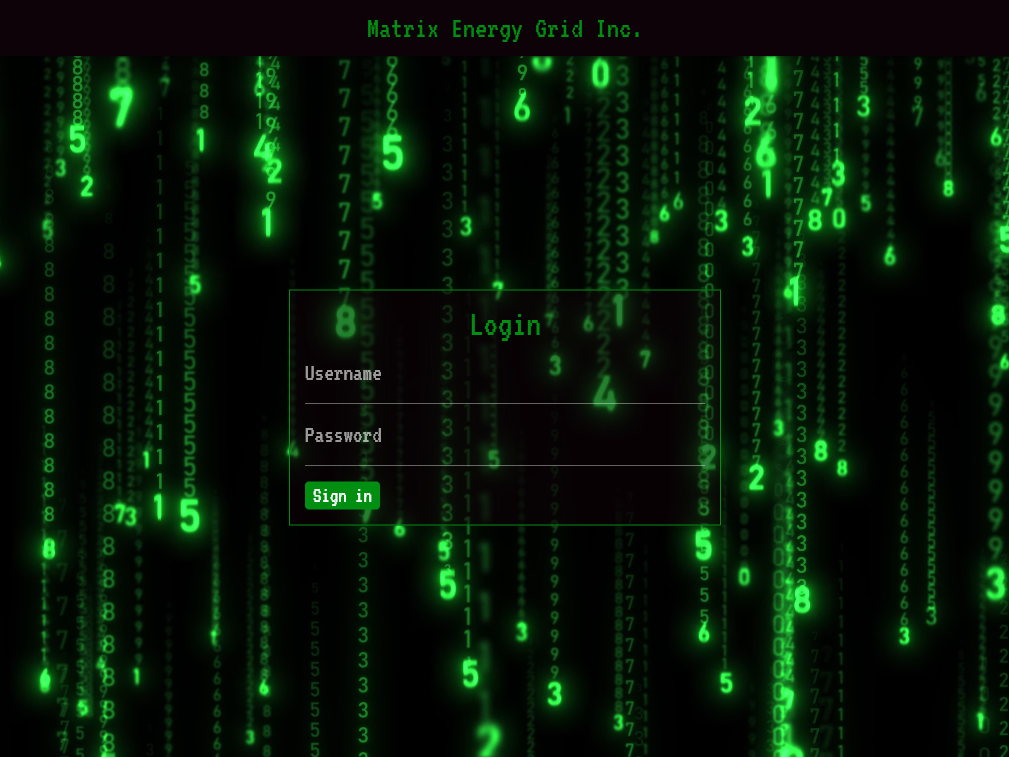
\includegraphics[width=.7\textwidth]{img/login.png}
    \caption{Anmeldebildschirm unter Port 80}
\end{figure}

Es gibt mehrere Möglichkeiten, an die Zugangsdaten zu gelangen. Der einfachste Weg wäre, einen Blick auf den HTML-Quelltext der Website zu werfen, welcher \blockquote{Test-Zugangsdaten} enthält oder einen Bruteforce-Angriff durchzuführen, welcher dadurch erleichtert wird, dass das Backend in der Rückmeldung angibt, ob Passwort oder Benutzername falsch waren, und sowohl Benutzername als auch Passwort weit oben in der \texttt{rockyou.txt} erscheinen.

\begin{lstlisting}[language=HTML]
<!DOCTYPE html>
<!--
FOR TESTING ONLY!!!
Credentials:
Username: smithy
Password: 010101
-->

<html>
\end{lstlisting}

Nach der Eingabe der Zugangsdaten aus dem HTML-Quelltext erhält man Zugriff auf die Verwaltungsoberfläche der \enquote{Matrix Energy Grid Inc.}


\begin{figure}[!ht]
    \centering
    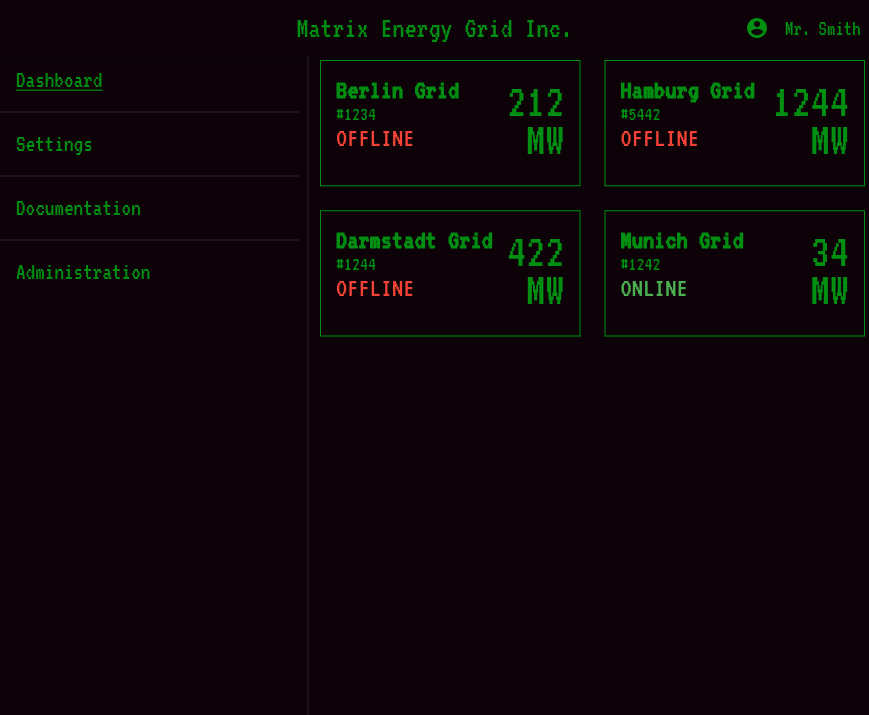
\includegraphics[width=.7\textwidth]{img/dashboard.png}
    \caption{Dashboard nach der Anmeldung}
\end{figure}

Unter dem Menüpunkt \blockquote{Settings} können nun Profilinformationen abgerufen werden. Dabei lässt sich feststellen, dass der eingeloggte Benutzer keine Administratorrechte hat. Ferner erlaubt die Seite die Änderung des Anzeigenamens.

\begin{wrapfigure}{r}{0.5\textwidth}
    \centering
    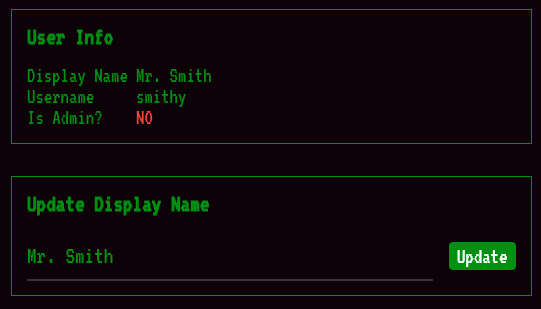
\includegraphics[width=.5\textwidth]{img/settings.png}
    \caption{Profileinstellungen}
\end{wrapfigure}

Das Verfahren zur Sitzungsverwaltung sieht zunächst sicher aus:
Angelehnt an JSON~Web~Tokens~(JWT) wird vom Server eine Payload-JSON generiert, die die Profilinformationen enthält.
Diese Payload wird über einen HMAC mit einem geheimen \texttt{SECRET} signiert und die Signatur dann anschließend zusammen mit der Payload als base64 in einem Cookie \texttt{MATRIXSESSION} gespeichert.
Bei weiteren Anfragen sendet der Browser den Cookie, und der Server überprüft nur die Signatur und kann vertrauen, dass die Profilinformationen in der Payload korrekt sind -- die Payload wurde schließlich vom Server selbst ausgestellt.
Der Signaturalgorithmus wird in der API-Dokumentation, die ebenfalls über die Webseite gelesen werden kann, beschrieben.

Mit der Implementierung eines eigenen kryptographischen Protokolls hat sich jedoch eine Schwachstelle aufgetan:
Für den HMAC wurde bcrypt als Hashfunktion verwendet.
Jedoch kann bcrypt Eingaben, die länger als 72~Bytes sind, nicht verarbeiten; überstehende Bytes werden ignoriert.
Effektiv deckt die Signatur also nur die ersten $(\hbox{72} - \hbox{\textit{Länge des \texttt{SECRET}}})$ Zeichen der Payload ab, die verbleibenen Zeichen können jedoch durch den Angreifer modifiziert werden, ohne dass die Signatur invalidiert wird.

Ein \texttt{MATRIXSESSION}-Cookie kann etwa wie folgt aussehen:
\begin{lstlisting}
eyJ1c2VybmFtZSI6InNtaXRoeSIsImRpc3BsYXlfbmFtZSI6Ik1yLiBTbWl0aCIsImlzX2FkbWluIjpmYWxzZX0=.JDJhJDEwJGs0OWcxL21ONTFUVUcuUmxlUnVvbnVNTmY2NHNEekJVVWx1dXBrZ25hUnJhdkZYTmFuWDNH
\end{lstlisting}

Rechts vom Punkt befindet sich der HMAC, links vom Punkt die Payload.
Diese dekodiert zu
\begin{lstlisting}[language=JSON]
{"username":"smithy","display_name":"Mr. Smith","is_admin":false}
\end{lstlisting}

\begin{wrapfigure}{r}{0.5\textwidth}
    \centering
    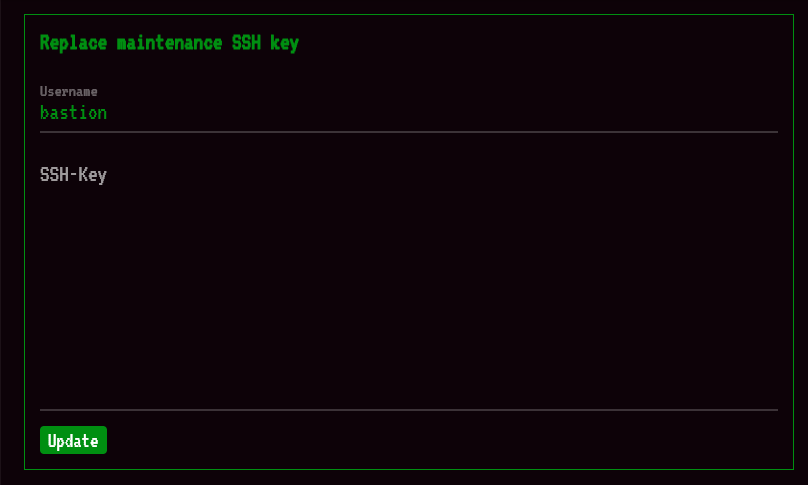
\includegraphics[width=.5\textwidth]{img/ssh.png}
    \caption{Hochladen des SSH-Key}
\end{wrapfigure}

Das Flag \texttt{is\_admin} ist der letzte Eintrag in der JSON.
Gelingt es also, zusammen mit dem unbekannten \texttt{SECRET} mindestens 72~Zeichen vor dem \texttt{false} einzufügen, dann wird diese Flag nicht von der Signatur abgedeckt und kann somit beliebig manipuliert werden.

Tatsächlich kann der \texttt{display\_name} über die Profileinstellungen geändert werden.
Das Frontend begrenzt zwar die Länge des Anzeigenamens, das Backend allerdings nicht.
So kann man einen neuen Cookie bekommen, bei dem ein entsprechend langer \texttt{display\_name} dafür sorgt, dass die Signatur eine Änderung von \texttt{is\_admin} auf \texttt{true} erlaubt.
Mit dem Admincookie erlangt man nun Zugriff auf das Admin-Panel, über das ein SSH-Key für den \texttt{bastion}-Linux-User hochgeladen werden kann.
Nach dem Login über SSH erscheint das erste Token in der Message~of~the~day:
\lstinputlisting{tokens/token1}

\subsection{Auslesen des Framebuffer}
Einer der ersten Schritte, die ein Angreifer nach Erlangen einer Shell durchführt, ist die Abfrage der User-ID über \texttt{id}.
Der Befehl zeigt an, dass der eingeloggte \texttt{bastion}-Benutzer Teil der \texttt{video}-Gruppe ist, die unter anderem das Lesen des Bildschirminhalts erlaubt.

Der Framebuffer kann über die Datei \texttt{/dev/fb0} ausgelesen und auf die eigene Maschine kopiert werden:
\begin{lstlisting}
ssh bastion@localhost "cat /dev/fb0" > fb0.raw
\end{lstlisting}

Anders als etwa JPEG- oder PNG-Bilder wird der Framebuffer nicht komprimiert gespeichert, sondern enthält Pixel für Pixel die einzelnen Werte für die Farbkanäle.
Ferner bedeutet das auch, dass die Auflösung nicht in der Datei enthalten ist.

An dieser Stelle kann die Auflösung entweder durch ausprobieren, durch Berechnungen auf Basis der Dateigröße oder mit dem Befehl \texttt{fbset} ermittelt werden:
\begin{itemize}
\item In den ersten beiden Fällen muss nur die Weite des Bildschirms geraten werden und die Höhe ergibt sich automatisch. Der Framebuffer ist etwa 1572864~Bytes groß, bei 16-bit Farbtiefe (das ist üblich bei Framebuffern) sind das 786432~Pixel. Mit der gerateten Weite von 1024~Pixeln ergibt sich eine Höhe von 786432 / 1024 = 768~Pixeln.
\item Im letzten Fall gibt \texttt{fbset} sowohl die Bildschirmgröße als auch die Kodierung zurück:
\begin{lstlisting}
mode "1024x768-0"
	# D: 0.000 MHz, H: 0.000 kHz, V: 0.000 Hz
	geometry 1024 768 1024 768 32
	timings 0 0 0 0 0 0 0
	accel true
	rgba 8/16,8/8,8/0,0/0
endmode
\end{lstlisting}
\end{itemize}

Um den Framebuffer nun sichtbar zu machen, bietet sich GIMP an, das bereits eine Funktion zum Lesen roher Bilddaten enthält.
Über eine schnelle Google-Suche sind allerdings auch einige fertige Python-Skripte zu finden, die den Framebuffer in eine PNG umwandeln können.

\begin{figure}[!ht]
\centering
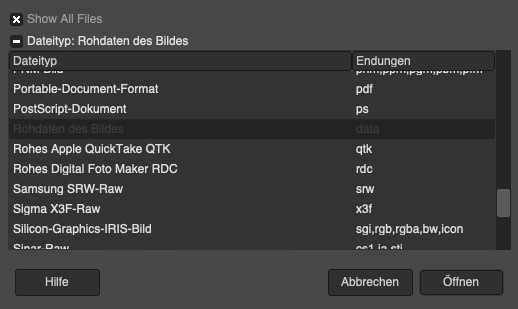
\includegraphics[width=.7\textwidth]{img/video_gimp_open.png}
\caption{Öffnen des Framebuffer als rohes Bild in GIMP}
\end{figure}

In einem neuen Fenster ist dann eine Vorschau des Framebuffer zu sehen, hier müssen jedoch noch die Dimensionen und die Kodierung spezifiziert werden.
Wenn noch nicht erfolgt, dann kann auch über das Vorschaufenster die Bildschirmgröße geraten bzw. ausprobiert werden.

\begin{figure}[!ht]
\centering
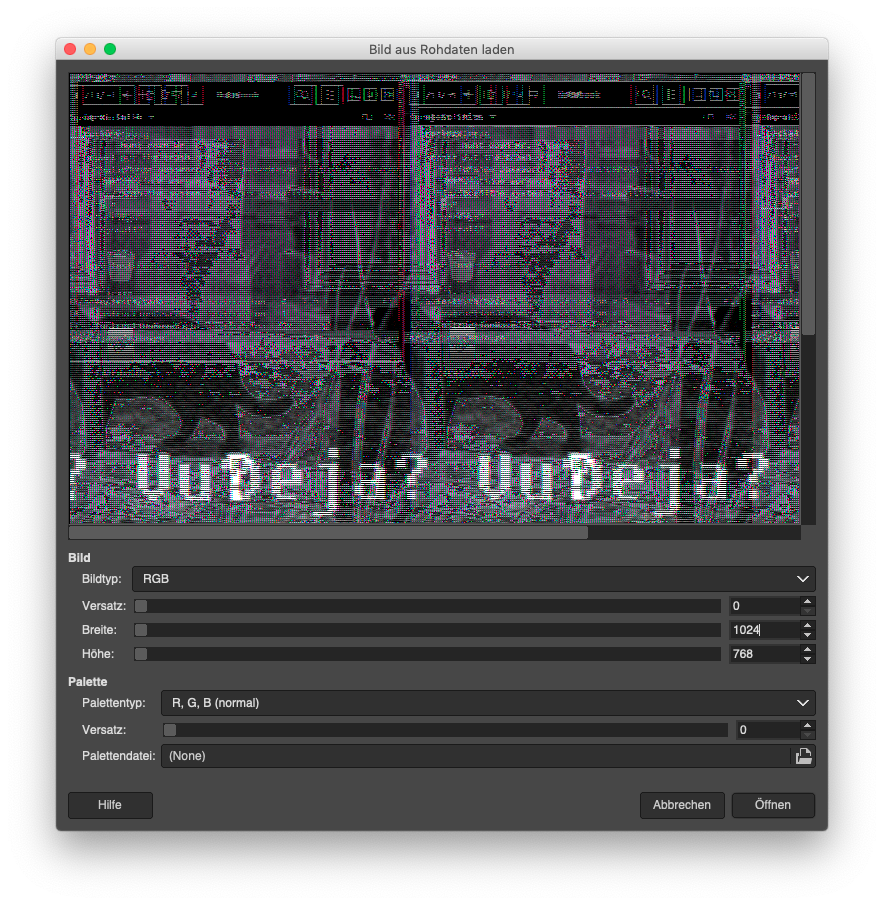
\includegraphics[width=\textwidth]{img/video_gimp_load.png}
\caption{Vorschau des Framebuffer}
\label{fig:video_gimp_load}
\end{figure}

In \cref{fig:video_gimp_load} wurde der Bildtyp bzw. die Kodierung noch nicht korrekt ausgewählt.
Hier kann auch entweder kurz durchprobiert oder die Kodierung aus \texttt{fbset} gelesen werden.
Häufig sind Framebuffer in RGB565 kodiert, wie auch hier, in diesem Fall in Little-Endian.

\clearpage
\begin{landscape}
\begin{figure}[!ht]
\centering
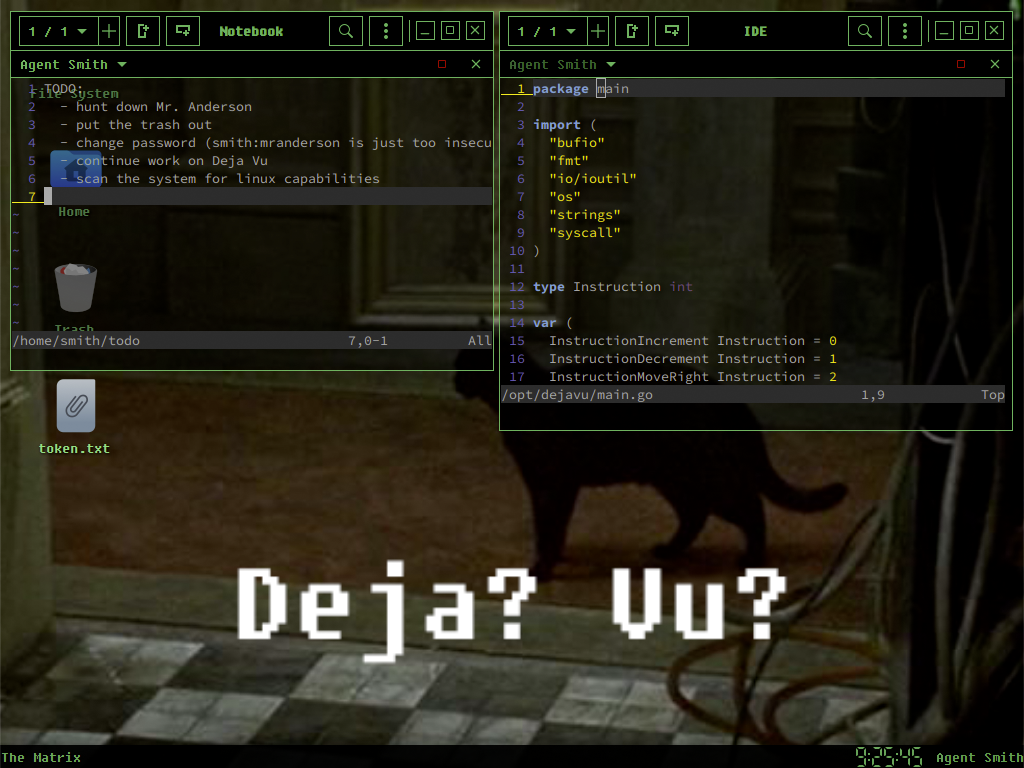
\includegraphics[height=\textwidth]{video/fb0.png}
\caption{Der Bildschirm, wie er im Framebuffer gespeichert ist}
\end{figure}
\end{landscape}
\clearpage

Prinzipiell wurde in dem Schritt also ein Screenshot gemacht, auf dem nun zu sehen ist, dass Agent~Smith eingeloggt ist.
Des Weiteren ist eine TODO-Liste geöffnet sowie der Quellcode von einem Programm.

Aus der TODO-Liste lässt sich ermitteln, dass Agent~Smith den Benutzernamen \texttt{smith} und das Passwort \texttt{mranderson} hat.

Im Screenshot finden sich weitere Hinweise (\enquote{Deja Vu} im TODO und Hintergrund sowie im Quellcode, Linux Capabilities), die aber erst für spätere Schritt interessant sind.

In einer neuen SSH Sitzung kann sich nun als Benutzer \texttt{smith} mit genanntem Passwort eingeloggt werden.
Die \texttt{/home/smith/Desktop/token.txt} enthält das folgende Token:
\lstinputlisting{tokens/token2}

\subsection{Exploit des \texttt{devlogin}}
Bei Agent Smith handelt es sich noch nicht um den root-Benutzer, es ist also eine weitere Privilegienerhöhung notwendig.
Nach kurzer Untersuchung des Dateisystems kann das Verzeichnis \texttt{/opt/devlogin} identifiziert werden, welches speziell der Gruppe der \texttt{agents}, die Gruppe des eingeloggten Benutzers, gehört.

Die Berechtigungen im Verzeichnis sind wie folgt gesetzt:
\begin{lstlisting}
dr-xr-x---    1 dev      agents        4096 Jul  1 23:48 .
drwxr-xr-x    1 root     root          4096 Jul  1 23:48 ..
-r-sr-x---    1 dev      agents       28008 Jul  1 23:33 devlogin
-r--r-----    1 dev      agents        1126 Jul  1 23:33 devlogin.cpp
\end{lstlisting}

Es liegt die setuid-Binary \texttt{devlogin} vor, welche bei der Ausführung die effektive UID auf die des Nutzers \texttt{dev} setzt.
Das Programm fragt nach Ausführung nach einem Benutzernamen und einem Passwort.
Ein kurzer Blick in den zugehörigen Quellcode verrät, dass der \texttt{devlogin} eine \texttt{dev}-Shell gibt, wenn die Zugangsdaten korrekt sind:
\lstinputlisting[linerange={36-44},firstnumber=36]{devlogin/devlogin.cpp}

Zudem kann aus dem Quellcode der beim Login gewünschte Benutzername (ebenfalls \texttt{dev}) sowie der MD5-Hash des Passworts (\texttt{14754f13e5280c5d49d2ae536c2d57e2}) entnommen werden.
Es lässt sich schnell ermitteln, dass das Passwort \texttt{machine} lautet.

Jedoch stellt man bei Eingabe dieser Zugangsdaten fest, dass immer noch keine Shell erzeugt wurde; das Problem:
Die Funktion, die zum hexadezimalen Kodieren des Passworthashes verwendet wurde, erzeugt einen Hexstring in Großbuchstaben und mit einem Doppelpunkt als Trennzeichen zwischen den Oktetten.
Der Zielhash hingegen ist in Kleinbuchstaben ohne Trennzeichen hinterlegt.
Es gibt also keine Möglichkeit, dass die Hexstrings identisch sein können.
Für eine Privilegienerhöhung muss also ein anderer Weg gefunden werden.

Im Rahmen der Challenge ist ein Exploit via \texttt{LD\_PRELOAD}-Umgebungsvariable vorgesehen, die den dynamischen Linker dazu bringt, eine benutzerdefinierte Bibliothek zu laden.
Zufälligerweise ist im Docker-Image bereits ein C-Compiler vorinstalliert, sodass die Bibliothek direkt im Container selbst erzeugt werden kann.
Dazu wird eine C-Datei \texttt{inject.c} mit folgendem Inhalt angelegt (\hbox{z. B.} im \texttt{/tmp}-Verzeichnis mit \texttt{vi}):
\lstinputlisting[language=C,linerange={1-8}]{devlogin/ld_preload.txt}

Die \texttt{\_init}-Funktion wird aufgerufen, sobald die dynamische Library geladen wurde, und ersetzt den aktuellen Prozess durch eine Shell.
Das \texttt{unsetenv} stellt lediglich sicher, dass die Bibliothek nicht in einer Endlosschleife sich selbst lädt.
Anschließend wird der Code mit folgendem Befehl in eine dynamische Bibliothek kompiliert:
\lstinputlisting[linerange={10}]{devlogin/ld_preload.txt}

Die Privilegienerhöhung erfolgt anschließend durch setzen von \texttt{LD\_PRELOAD} auf die kompilierte Bibliothek vor der Ausführung des \texttt{devlogin}-Programms:
\begin{lstlisting}
$ id
uid=1000(smith) gid=1000(agents) groups=27(video),1000(agents),1000(agents)
$ LD_PRELOAD=/tmp/inject.so ./devlogin
$ id
uid=1002(dev) gid=1000(agents) groups=27(video),1000(agents),1000(agents)
\end{lstlisting}

Mit Shell-Zugriff zum \texttt{dev}-Benutzer kann auch das nächste Token unter \texttt{/home/dev/token.txt} gelesen werden:
\lstinputlisting{tokens/token3}

Nun ist es verwunderlich, dass \texttt{LD\_PRELOAD} auf einer setuid-Binary funktioniert, wie das Token auch andeutet.
Tatsächlich wird die eigene Bibliothek nicht in den \texttt{devlogin} injiziert, sondern in den Kindprozess, der in Zeile~18 erzeugt wird:
\lstinputlisting[language=C,linerange={13-19},firstnumber=13]{devlogin/devlogin.cpp}
Das Docker-Image ist ein musl-basiertes System, d.h. alle Binaries benutzen den dynamischen Musl-Linker.
Dies kann über den \texttt{file}-Befehl auf der Binary verifiziert werden.
Anders als der GNU dynamische Linker\footnote{\url{https://github.com/bminor/glibc/blob/master/sysdeps/generic/unsecvars.h\#L22}} löscht musl \textbf{nicht} die \texttt{LD\_PRELOAD}-Umgebungsvariable bei setuid-Binaries, sondern ignoriert diese lediglich.
Sie wird also trotzdem an Kindprozesse weitergegeben.
Voraussetzung ist nur, dass die echte UID mit der effektiven UID übereinstimmt\footnote{\url{https://github.com/esmil/musl/blob/master/src/ldso/dynlink.c\#L1121-L1123}}, dafür sorgt Zeile 14.
Eine korrekte Implementierung würde den Code in Zeile~14 erst nach erfolgreichem Login in Zeile~42 durchführen.

\subsection{Privilege Escalation via Deja Vu}
Der Benutzer \texttt{dev} hat Zugriff auf das Verzeichnis \texttt{/opt/dejavu}, aus dem bereits im Screenshot von Agent Smith eine Datei geöffnet war.

In dem Verzeichnis findet sich ein Interpreter für die Deja Vu Programmiersprache, welche die Maschinen zur Programmierung von künstlicher Intelligenz einsetzen -- zurzeit jedoch nur in Katzenprogrammen, wie in der beiliegenden \texttt{README.md} angemerkt wird.

\begin{lstlisting}
dr-xr-x---    1 dev      dev           4096 Jul  4 10:22 .
drwxr-xr-x    1 root     root          4096 Jul  4 10:22 ..
-r--r-----    1 dev      dev           1657 Jun 30 09:20 README.md
-r-xr-x---    1 dev      dev        2034928 Jul  4 10:21 dejavu
dr-xr-x---    1 dev      dev           4096 Jul  4 10:22 examples
-r--r-----    1 dev      dev           4980 Jul  3 09:58 main.go
\end{lstlisting}

Ferner enthält die \texttt{README.md} eine kurze Übersicht der erlaubten Instruktionen sowie einen Verweis auf Beispiel-Skripts im \texttt{examples}-Verzeichnis.
Bei Deja Vu handelt es sich um eine Abwandlung der esoterischen Programmiersprache Brainfuck bzw. deren Variante \href{https://de.wikipedia.org/wiki/Ook!}{Ook!}

Nach einem kurzen Blick in den ebenfalls beiliegenden Quellcode kann festgestellt werden, dass eine weitere, undokumentierte Instruktion unterstützt wird, welche das Ausführen externer Programme ermöglicht; jedoch erschließt sich ein möglicher Angriff erstmal nicht, denn der Interpreter ist keine setuid-Binary, wird also ganz normal als Benutzer \texttt{dev} ausgeführt.
Jedoch findet man nach ausführlicher Untersuchung heraus, dass die Interpreter-Binary die Linux~Capability \texttt{CAP\_SETFCAP} über die erweiterten Dateisystem-Attribute gesetzt hat, darauf gab es bereits in der TODO-Liste im Screenshot einen Hinweis.

\begin{lstlisting}
$ getcap dejavu
dejavu cap_setfcap=eip
\end{lstlisting}

Die \texttt{CAP\_SETFCAP}-Capability erlaubt dem ausgeführten Interpreter-Prozess beliebiges Setzen weiterer Capabilities im Dateisystem.
Mehrere Wege führen hier zum Ziel, in diesem Walkthrough wird die \texttt{CAP\_DAC\_OVERRIDE}-Capability der \texttt{/bin/busybox} zugewiesen, wodurch für alle Busybox-Tools wie \texttt{ls} oder \texttt{cat} die Rechteüberprüfung auf Dateisystemebene deaktiviert wird.

Normalerweise würde ein Administrator dazu folgenden Befehl ausführen:
\begin{lstlisting}
$ /usr/sbin/setcap cap_dac_override+eip /bin/busybox
unable to set CAP_SETFCAP effective capability: Operation not permitted
\end{lstlisting}

Mit dem passenden DejaVu-Skript sollte dieser Befehl aber erfolgreich ausgeführt werden.
Dieses Skript wird am besten automatisiert generiert, denn die undokumentierte Instruktion (\texttt{Deja? Vu?}) zum Ausführen eines Programms erfordert, dass die Zelleninhalte relativ zum Zeiger in einer bestimmten Struktur vorliegen.
Demnach steht in der ersten Zelle die Länge des ersten Zeichenkette, gefolgt von dieser Zeichenkette (pro Zelle ein Byte).
In der nächsten Zelle steht dann die Länge der zweiten Zeichenkette, gefolgt von der zweiten Zeichenkette.
Die Argumentliste terminiert bei einer 0.

\begin{figure}[!ht]
\centering
\begin{tikzpicture}
\matrix[
    matrix of nodes,
    every node/.style={
        draw,
        anchor=center,
        minimum height=20pt,
        minimum width=20pt,
        text=blue
    }
]{
    \strut \color{red}9 & \strut / & \strut b & \strut i & \strut n & \strut / & \strut e & \strut c & \strut h & \strut o &
    \strut \color{red}5 & \strut H & \strut a & \strut l & \strut l & \strut o &
    \strut \color{red}0 \\
};
\end{tikzpicture}
\caption{Struktur der Zellen mit \texttt{/bin/echo Hallo} als Beispiel}
\end{figure}

Der folgende JavaScript-Code generiert ein DejaVu-Skript, welches den gewünschten \texttt{setcap}-Befehl korrekt in die Zellen organisiert und die undokumentierte Instruktion ausführt:

\lstinputlisting[language=JavaScript]{dejavu/buildDejavu.js}

Es wird ein ca.~50000-Zeichen langes DejaVu-Skript generiert, welches anschließend auf die Maschine als \texttt{/tmp/exploit.dv} kopiert und mit dem Interpreter ausgeführt werden kann:

\begin{lstlisting}
$ whoami
dev
$ ls /root
ls: can't open '/root': Permission denied
$ ./dejavu /tmp/exploit.dv
$ whoami
dev
$ ls /root
token.txt
$ cat /root/token.txt
HC2021{WhoEvenNeedsRootWhenThereAreCaps}
\end{lstlisting}


\clearpage
\section{Bemerkungen}
\subsection{Schwierigkeitsgrad}
An einigen Stellen in der Challenge mussten wir abwägen, wie leicht oder schwierig wir einen Schritt gestalten, wie viele Hinweise wir geben und wie viel Zeit ein Schritt erfordert.

So wurden beispielsweise im ersten Schritt die Zugangsdaten direkt in die HTML-Datei geschrieben.
Ein Bruteforcing wäre zwar in relativ kurzer Zeit möglich gewesen, halten wir aber als ersten Schritt für demotivierend und einen geringen Lerneffekt.

Des Weiteren findet sich im Screenshot ein Hinweis auf die Linux~Capabilities.
Diesen haben wir eingebaut, da wir vermuten, dass die meisten Studenten (die ja in der Lage sein sollen, diese Challenge zu lösen) wenig vertraut mit diesem Linux-Feature sind bzw. möglicherweise dieses garnicht kennen.
Ein Privilege-Escalation-Skript wie \texttt{linpeas.sh} findet die gesetzte Capability jedoch.

Ferner wäre auch ein Weglassen des \texttt{dejavu}-Quellcodes möglich gewesen, mit entsprechend benötigtem Zeitaufwand für diesen Schritt.

\subsection{Limitierungen}
Im Framebuffer-Schritt wird kein echter Framebuffer (das wäre ein Character-Device) gedumpt, sondern nur eine readonly-Datei mit identischen Berechtigungen. 
Das liegt daran, dass der Docker-Container nicht die nötigen Privilegien besitzt, um ein \texttt{devfs} mit einem eigenen Framebuffer-Device zu mounten.
Auch können wir dadurch leider nicht die Bildschirmauflösung in \texttt{sysfs} ausgeben; es bleibt ein überschriebenes \texttt{fbset}-Programm mit statischer Ausgabe.

\end{document}
